\chapter{Introduction}
This documentation contains information about the specifications, design, architecture and functionality of the electrically propulsed car named 'AU2'. This system has been designed to be able to compete in Shell Eco Marathon (in the Prototype - Battery-electric category).

\begin{figure}[H]
	\centering
	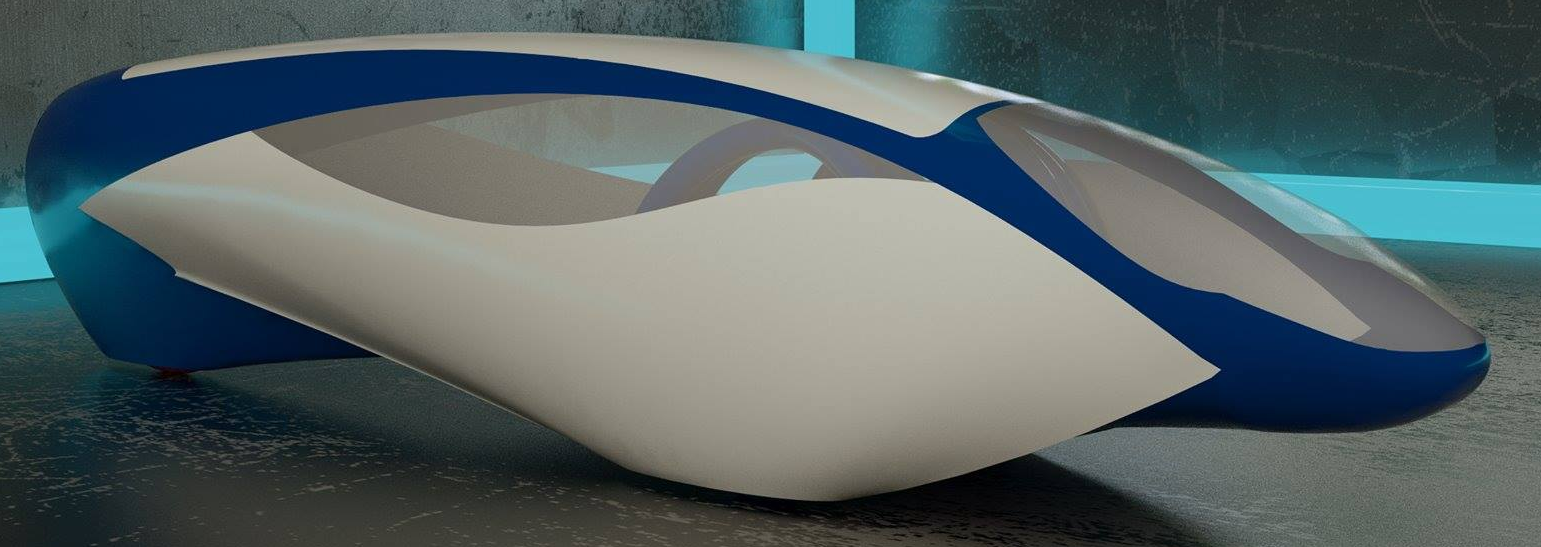
\includegraphics[width=0.5\linewidth]{Introduction/Model}
	\caption{Computer generated model of the car}
	\label{fig:System_model}
\end{figure}

\section{System description}
The primary purpose of the car is to be as energy-effecient as possible, as this is the goal of Shell Eco Marathon. This has been acheived by implementing a optimized driving-algorithm \fxnote{Kunne dette uddybes? Og hvad med hardware?}.

\section{List of terms}
The following list explains the various terms which has been used to refer to certain parts or subsystem in this documentation.

\begin{itemize}
	\item \textbf{SEM}\\
	Refers to Shell Eco Marathon which the car is designed to compete in.
\end{itemize}